\documentclass[12pt, class=report, crop=false]{standalone}
\usepackage{ba_thesis}

\begin{document}

\chapter{Plasma Physics}%
\label{chap:plasma}

\section{The Definition of Plasma}
It is common that people, when asked about what is plasma, their definition stops at the fact that it is a \textbf{partially ionized gas}. But this is just one of the three defining characteristics. After all, even the air is partially ionized. The other two proprties that a medium should satisfy in order to be considered plasma are quasi-neutrality and collective behaviour.

To be \textbf{quasi-neutral} means that the medium has an equal number of positive and negative charges in its entire volume, but small deviations from neutrality are possible locally. That is, if \(n_p\), \(n_e\) are the positive charge density and the electron density, respectively, in the whole region of the plasma we have \(n_p = n_e\), yet in small regions in the space inside we have \(n_p \approx n_e\). A small remark should be made here. While I say that the plasma as a whole is neutral, it is so by approximation still. If one starts building plasma by pumping energy into a gaseous medium for example, some of the first ionized electrons can actually escape the medium. It is only after a certain positive charge density has been achieved that no electrons can not escape anymore due to Coulomb attraction. Once enough ionization electrons are produced, the charge imbalance becomes incredibly small (\textit{i}.\textit{e}. \(\frac{n_p - n_e}{n_e}\ll 1\)). This is though a very hard to observe charge imbalance in practice, so we can say that plasma as a whole is neutral. The localized imbalance in turn is not constantly small; it can vary widely due to the disordered motion of the constituent particles, but statistically speaking neutrality is maintained locally when we look at the time averages.

\textbf{Collective behaviour} is a consequence of the fact that the main type of interaction between the particles constituting the plasma, namely Coulomb interaction, is long range. As such, we can say that any particle in the plasma feels all the other ones. This leads to many important properties specific to plasma, like particle and momentum transport. The simplest response is plasma oscillation, which arises when plasma is placed in a constant electric field. The electrons are pushed by the electric field, but the surplus of positive charge left behind pulls them back, creating an oscillatory motion (we should take into consideration that the positive ions are at least a couple thousand times heavier than the electrons, so it is harder to influence their motion).This property also influences the the way in which plasma interacts with electromagnetic radiation, giving rise to radiation transport phenomena for example.

It is important to note from the very begining that in a plasma we have quite many different species of particles. The most simple model would only include electrons, neutral atoms and ions that have just one missing electron, but in reality we can have all the possible types of ions (so also with two or more missing electrons) and photons (which arise from the excitations and de-excitations that happen in this very energetic medium).

In the following sections we aim to go deeper into the parameters that characterize plasmas and the basic models for it. The discussion brings together ideas from~\cite{karschApplicationsHighIntensity2018} and~\cite{mulserHighPowerLasermatter2010}.

\section{Temperature}
We would like now to study the statistics of electrons. First of all, we should realize that the interparticle distances in plasmas are quite large, but also the temperature needed to sustain ionization is quite high. So high in fact that working with the Fermi-Dirac statistics is not necesary, since this quantum mechanically derived distribution can be approximized very well by the classical Maxwell-Boltzmann distribution in this particular situation.

The number of electron with x-axis velocity between \(v_{e,x}\) and \(v_{e,x}+\dd{v_{e,x}}\) is then given by

\begin{equation}
  f_e (v_{e,x}) \dd{v_{e,x}} = n_e \sqrt{\frac{m_e}{2\pi K_B T_e}} \ee^{-\frac{K_x}{K_B T_e}}\,,
\end{equation}
where \(n_e\), \(m_e\) and \(T_e\) are the electrons' density, mass and temperature, respectively, \(K_B\) is the Boltzmann constant and \(K_x = \frac{m_e v_{e,x}^2}{2}\) is the kinetic energy of the photons. The normalization constant was obtained from the electron density, since \(n_e = \int_{-\infty}^{+\infty} \dd{v_{e,x}} f_e (v_{e,x})\). This gives an average kinetic energy of

\begin{equation}
  K_x^{avg} = \frac{\int_{-\infty}^{+\infty} \dd{v_{e,x}} K_x f_e (v_{e,x})}{\int_{-\infty}^{+\infty} \dd{v_{e,x}} f_e (v_{e,x})} = \frac{m_e}{2 n_e} \int_{-\infty}^{+\infty} \dd{v_{e,x}} v_{e,x}^2 f_e (v_{e,x}) = \frac{1}{2} K_B T_e\,.
\end{equation}

This is extended in 3D easily, since the distribution of velocity in this case should not have any preferential direction

\begin{equation}
  K^{avg} = \frac{3}{2} K_B T_e\,.
\end{equation}
As it can be seen, we can basically treat the electrons inside the plasma as we would an ideal gas and we have obtained that the average kinetic energy is proportional to the temperature.

A simple numerical application shows us that in order to have \(K_B T_e = 1\) eV, the temperature would be around \(11600\) K. Thus, since the ionized electrons are above the energy level of outer bounded states (so above 1 eV), using Kelvin or degrees Celsius is not that handy. In practice, we will rather use eV (energy units) temperature, which is to be converted to the usual temperature by dividing to \(K_B\).

We could actually treat the ions and the neutral atoms inside the plasma in the same manner. Considering this, we must make the remark that we can have different temperature scales in plasmas. While at thermodynamic equilibrium the system of electrons, ions and neutrals should have a uniform temperature, under the action of an electric field, lets say, the motion of the electrons is influenced more than that of the ions due to the difference in mass, while the neutrals are not affected at all, so we have \(T_n\neq T_i\neq T_e\). Of course, equilibration between species can be achieved through collisions or radiation emission and absorption. In complete models, one should also consider the temperatures of photons and individual ion subspecies that can appear. Considering this, in general, thermal equilibration can take a long time (How long exactly is hard to say. Even a rough estimate should account for many types of collisions that take place in a plasma. A comperhensive list of the processes occuring can be found in~\cite{braithwaiteIntroductionGasDischarges2000}). It is also important to visualize that the temperature can be directional depending on the orientation of the fields we apply.

Regarding the photons in the system, we must point out that they never reach an equilibrium state. That is because photons are not maintained in the plasma like the other forces (say, electrons and ions pulled back in the plasma by Coulomb forces, neutral particles which have to deal with surface effects). This effect is easy to see in practice. Since the photons leave the plasma medium, the plasma itself is radiating light. This property is the basis for building plasma lamps and plasma displays.

\section{Debye Shielding}
In this section we will derive a common criterion for quasi-neutrality. Let us consider an infinite medium filled with plasma at thermal equilibrium, \(T=T_e = T_i\) and with one ion species with charge \(Ze\), such that we have \(n_e = Zn_i\). We are interested to see what happens if we introduce an infinite plane with constant positive surface charge density \(\sigma\) in this system (see~\cref{fig:debye}).

\begin{figure}[h]
  \centering
  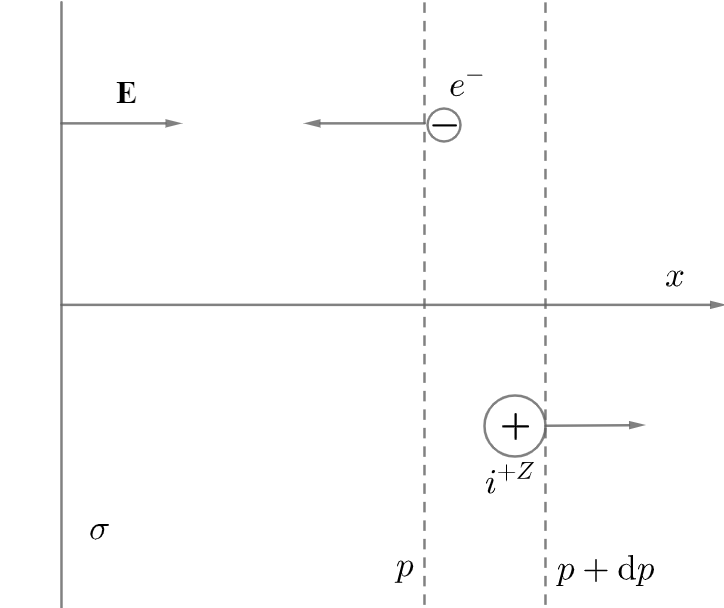
\includegraphics[width=0.52\textwidth]{Debye}%
  \caption{A schematic figure that shows the action of introducing the charged sheet in the plasma}\label{fig:debye}%
\end{figure}

The constant electric \(E = \frac{\sigma}{2\varepsilon_0}\) generated by the plate will act to locally separate sheets of electrons and ions, until equilibrium between the pressures \(p_e = n_e K_B T\) and \(p_i = n_i K_B T \) is achieved. For the electrons in a sheet of thickness \(\delta x\) we have

\begin{equation}
  \dd{p_e} = K_B T \dd{n_e} = -e n_e E \delta x\,,
\end{equation}
which can be rewritten as

\begin{equation}
  \frac{1}{n_e} \partial_x n_e = - \frac{e}{K_B T} E = \frac{e}{K_B T} \partial_x \phi\,,
\end{equation}
where \(\phi\) is the electrostatic potential. Solving this equation for the density of electrons, we obtain

\begin{equation}
  n_e(x) = \bar{n}_e \ee^{\frac{e\phi}{K_B T}},\; \bar{n}_e = n_e(x \rightarrow \infty)\,.
\end{equation}
In the same manner one obtains a similar expression for the ion density

\begin{equation}
  n_i (x) = \frac{\bar{n}_e}{Z} \ee^{-\frac{Ze\phi}{K_B T}}\,.
\end{equation}

Writing the Poisson equation in terms of these results gives us

\begin{equation}
  \partial_x^2 \phi = \frac{e \bar{n}_e}{\varepsilon_0} \left(\ee^{\frac{e\phi}{K_B T}} - \ee^{-\frac{Ze\phi}{K_B T}} \right)\,.
\end{equation}
If the potential energy arising from the field is small compared the the kinetic energy of the particles in the plasma, \textit{i}.\textit{e}. \(e\phi\ll K_B T\), the potential equation can be simplified in approximation to

\begin{equation}
  \partial_x^2 \phi = \frac{e \bar{n}_e}{\varepsilon_0} \left( 1 +\frac{e\phi}{K_B T} -1 + \frac{Ze\phi}{K_B T}\right) = \frac{e^2 \bar{n}_e (Z+1)}{\varepsilon_0 K_B T} \phi\,.
\end{equation}
Obtaining the solution if this is trivial

\begin{equation}
  \phi(x) = \phi_0 \ee^{-\frac{x}{\lambda_D}}\,,
\end{equation}
where we introduced the Debye length

\begin{equation}
  \lambda_D = \sqrt{\frac{\varepsilon_0 K_B T}{\bar{n}_e e^2 (Z+1)}}\,.
\end{equation}
This shows us that at a distance of \(\lambda_D\) away from the plate, the electric field generated by it, as well as the corresponding potential, is screened by about 63\%. This offers us great insight in how to obtain quasi-neutrality.

From this discussion we can conclude that quasi-neutrality holds if the spatial extension of our ionized gas is at least a couple times larger than the Debye length, since in this case the local deviations from neutrality \(n_p\approx n_e\) are screened. For dimensions smaller than \(\lambda_D\), there is no quasi-neutrality very high-intensity localized fields can occur giving rise to interesting physical phenomena.

In practice, one uses another form for \(\lambda_D\) which neglects the \(Z\) and uses the temperature and particle density with more convenient units

\begin{equation}
  \label{def:debye-length}
  \lambda_D = \sqrt{\frac{\varepsilon_0 K_B T}{\bar{n}_e e^2}} = 6.9 \sqrt{\frac{T_e [\textrm{K}]}{n_e [\textrm{cm}^3 ]}}\,,
\end{equation}
the last expression giving \(\lambda_D\) in cm.

\section{Plasma Frequency}

The simplest plasma wave is a longitudinal oscilation of the electrons (caused by an external electric field). Considering how heavy all the other particle species are compared to them, we can treat this problem by considering the ions stationary. Thus, the electrons simply move in a static positive background. The local changes in electron density cause imbalance and, as we mentioned before, restoring Coulombian forces arise. In what follows we will work purely electrostatic by considering that the electric field is always paralel to the x-axis and the external electric field. We also consider that the electron temperature is close to zero.

We make use of the equation of motion for a single electron, the continuity equation and the Poisson equation

\begin{subequations}
  \begin{align}
    \label{eq:motion-plasma-freq}
    m_e \dv{v_x}{t} = m_e \left(\partial_t v_x + v_x \partial_x v_x\right) = -e E\\
    \label{eg:cont-plasma-freq}
    \partial_t n_e + \partial_x (n_e v_e) = 0\\
    \label{eq:poisson-plasma-freq}
    \partial_x E = \frac{e}{\varepsilon_0} (n_p - n_e)\,,
  \end{align}
\end{subequations}
where \(n_p\) is the positive charge density divided by the unit charge. In~\cref{eq:motion-plasma-freq} we can neglect the second term by considering that the velocity is small. We have \(v_x \partial_x v_x = \frac{1}{2} \partial_x v_x^2 \approx 0\), since \(v_x^2\ll v_x\) (remember that we work with \(T_e\approx0\)), so

\begin{equation}
  \partial_t v_x = - \frac{e}{m_e} E\,.
\end{equation}
Similarly, considering that the particle density is also slowly changing around an equilibrium position \(n_0 = n_p\) (\textit{i}.\textit{e}. \(n_e = n_0 +n(x,t)\)), we can simplify~\cref{eg:cont-plasma-freq}

\begin{equation}
  \partial_t n_e + n_0 \partial_x v_x = 0\,.
\end{equation}
These approximations also change~\cref{eq:poisson-plasma-freq}

\begin{equation}
  \partial_x E = - \frac{e}{\varepsilon_0} n\,.
\end{equation}
Using a plane wave ansaz for \(E\), \(v_x\) and \(n\)

\begin{subequations}
  \begin{align}
    E = E_0 \ee^{\ii(kx -\omega t)}\\
    v_x = v_0 \ee^{\ii(kx -\omega t)}\\
    n = n_{10} \ee^{\ii(kx -\omega t)}\,,
  \end{align}
\end{subequations}
The approximated equation become

\begin{subequations}
  \begin{align}
    -\ii\omega v_0 = - \frac{e}{m_e} E_0\\
    - \ii \omega n_{10} +\ii n_0 k v_0 = 0\\
    \ii k E_0 = - \frac{e}{\varepsilon_0} n_{10}\,.
  \end{align}
\end{subequations}
The frequency \(\omega\) can be extracted from these relations as follows

\begin{equation}
  -\ii\omega v_0 = - \frac{e}{m_e} E_0 =  \frac{e^2}{\ii \varepsilon_0 k m_e} n_{10} = \frac{e^2}{\ii \varepsilon_0 k m_e} \frac{k n_0}{\omega} v_0\,,
\end{equation}
or

\begin{equation}
  \label{def:plasma-frequency}
  \omega_p = \sqrt{\frac{n_0 e^2}{\varepsilon_0 m_e}}\,.
\end{equation}
This is called the cold plasma frequency. This result can be used to derive the plasma waves dispersion relation for the thermal motion of electrons

\begin{equation}
  \omega^2 = \omega_p^2 + 3 k^2 \frac{K_B T_e}{m_e} = \omega_p^2 + \frac{3}{2} k^2 v_{th}^2\,,
\end{equation}
where \(v_{th}\) is the thermal velocity. As usual, the dispersion relation is useful for finding the phase and group veloities

\begin{subequations}
  \begin{align}
    v_{ph} = \frac{\omega}{k} = \sqrt{\frac{\omega_p^2}{k^2} + \frac{3}{2} v_{th}^2} \\
    v_{gr} = \pdv{\omega}{k} = \frac{3}{2} \frac{v_{th}^2}{v_{ph}}\,.
  \end{align}
\end{subequations}
All these velocities satisfy the inequality

\begin{equation}
  v_{gr} < \sqrt{\frac{3}{2}} v_{th} < v_{ph}\,.
\end{equation}

It is also important to remark that the cold plasma frequency~(\ref{def:plasma-frequency}) and the Debye length~(\ref{def:debye-length}) can be related with each other

\begin{equation}
  \omega_p \cdot \lambda_D = \sqrt{\frac{K_B T_e}{m_e}} \propto v_{th}\,.
\end{equation}

\section{Electromagnetic Waves in Plasma}

We will now try to discuss how a plane wave interacts with a plasma medium. We shall start assumung that we have a wave that enters the plasma having initially the properties

\begin{subequations}
\label{plasma-plane-wave}
  \begin{align}
    \vb{E},\, \vb{B}\propto \ee^{\ii (\vb{k}\vb{r}-\omega t)} \\
    \vb{B} = \frac{1}{c} \vb{k}\cp\vb{E}\,.
  \end{align}
\end{subequations}
For simplicity, we will assume that no longitudinal field components arise from the interaction with the plasma. While this may not be a perfectly realistic assumtion, the longitudinal components that appear would be very small and would not affect to much the result we obtain.

We will make use of the already familiar Maxwell equations (two of them, to be precise)

\begin{subequations}
  \begin{align}
    \curl{\vb{B}} = \mu_0\vb{j} +\frac{1}{c^2} \partial_t \vb{E} \Rightarrow \curl{(\partial_t \vb{B})} = \frac{1}{\varepsilon_0 c^2} \partial_t \vb{j} + \partial_t^2 \vb{E}\\
    \curl{\vb{E}} = - \partial_t \vb{B} \Rightarrow \curl{(\curl{\vb{E}})} = \grad{(\div{\vb{E}})} - \laplacian{\vb{E}} = - \curl{(\partial_t \vb{B})}\,.
  \end{align}
\end{subequations}
Bringing these results together gives

\begin{equation}
  \grad{(\div{\vb{E}})} - \laplacian{\vb{E}} + \frac{1}{\varepsilon_0 c^2} \partial_t \vb{j} + \partial_t^2 \vb{E} = 0\,.
\end{equation}
From~\cref{plasma-plane-wave} we can compute the derivatives to obtain

\begin{equation}
  \ii \grad{(\vb{k}\vdot\vb{E})} + k^2 \vb{E} - \ii \frac{\omega}{\varepsilon_0 c^2} \vb{j} - \frac{\omega^2}{c^2} \vb{E} = 0\,.
\end{equation}
Here the assumption of no longitudinal field component comes in handy and removes the first term, leaving us with
 \begin{equation}
   (\omega^2 - c^2 k^2)\vb{E} = -\ii \frac{\omega}{\varepsilon_0} \vb{j}\,.
 \end{equation}
We shall deviate a bit in order to find an expression for the current density. We can find the average electron velocity from the force equation

\begin{equation}
  m_e \partial_t \vb{v_e} = - e \vb{E} \Rightarrow \vb{v_e} = \frac{e}{\ii \omega m_e}
\end{equation}
and introduce it in the definition of the current density in terms of drift velocity

\begin{equation}
  \vb{j} = -e n_0 \vb{v_e}\,.
\end{equation}

By putting together these last three results we obtain the dispersion relation for plane electromagnetic waves in plasma

\begin{equation}
  \omega^2= \omega_p^2 +k^2c^2\,.
\end{equation}
From this, obtaining also the phase velocity is trivial

\begin{equation}
  v_{ph} = \frac{c}{\sqrt{1-\frac{\omega_p^2}{w^2}}} = \frac{c}{\eta}\,.
\end{equation}
Here we have also defined the plasma refractive index \(\eta = \frac{kc}{\omega}\). It gives very important criteria for propagation of waves in plasma. If \(\omega >\omega_p\), then \(\eta<1\) and the wave can propagate through. Otherwise, when \(\omega<\omega_p\) and \(\eta\) is imaginary, the wave can not propagate; it will drop exponentially after it enters the plasma medium. The group velocity is also obtained to be

\begin{equation}
  v_{gr} = c\eta < c\,.
\end{equation}
There is also a physical way to think about the possibility of propagation of a wave. If the electromagnetic oscillation occur at a faster rate than that to which the plasma can react, the charged particles in the plasma will not respond fast enough to shield the radiation and it will penetrate. In the oposite case, the incoming radiation is shielded and energy conservation dictates that the wave must be relfected. Whatever small part of the wave would enter the plasma will drop very fast.

\section{The Vlasov Equation}

There is an alternative way to treat the statistics of plasma populations without using the Maxwell-Boltzmann distribution. More precisely, one can derive an equation for the distribution function in phase space. In order to do that, we must start from the Liouville theorem~(\cite{arnoldMathematicalMethodsClassical1997}, p. 68).

\subsubsection{Theorem(Liouville)}
  The \textit{phase flow} is the one-parameter group of transformations of phase space
  \(g^t:(\vb{p}(0),\vb{q}(0))\rightarrow(\vb{p}(t),\vb{q}(t))\), where \(\vb{p}(t)\) and \(\vb{q}(t)\) are solutions of the Hamilton equations. The phase flow preserves the volume of any region. That is, for any region \(D\), \(V(g^tD)=V(D)\).
\newline

In more layman terms, for a Hamiltonian system, the volume in phase space is conserved in time. In this theorem we also defined the time propagation transformation group \(\{g^t\}\). Before delving into the proof of Liouville's theorem let us see that \({g^t}\) is indeed a group (just as a warming up exercise).

Let \(g^{t_a}\,,g^{t_b}\in \{g^t\}\) three arbitrary transformations (the time \(t\) is just a real parameter) and \(\vb{v}\,,\vb{p}\) solutions of Hamilton's equations. For the closure property we have

\begin{equation*}
  (g^{t_a}\cdot g^{t_b}):(\vb{p}(0),\vb{q}(0)) \equiv g^{t_a}:(g^{t_b}:(\vb{p}(0),\vb{q}(0))) \equiv g^{t_a}:(\vb{p}(t_b),\vb{q}(t_b)) \equiv
\end{equation*}

\begin{equation*}
  \equiv (\vb{p}(t_b+t_a),\vb{q}(t_b+t_a)) \equiv g^{t_b+t_a}:(\vb{p}(0),\vb{q}(0))\,.
\end{equation*}
We can see from this that composing two transformations gives another transformation whose parameter is the sum of the parameters of the initial transformations. Now it is easy to argue that associativity holds because the parameters are real numbers and their addition is associative. The identity element is \(g^0\) and the inverve of the element \(g^t\) is \(g^{-t}\). Even more, this group is abelian. This is consistent to the physical reality of time evolution, since, starting from exactly the same initial conditions, progressing in time first up to \(t_a\) and then up to \(t_a+t_b\) is equivalent to progressing in time first up to \(t_b\) and then up to \(t_a+t_b\).

Now let us turn back to proving the theorem. I will deonote by \(V(t)\) the volume of \(D(t)\), where \(D(t) = g^t D\) and \(D\) is the initial volume. Supposing we have the set on \(n\) ordinary differential equations

\begin{equation}
  \vb{u} = \vb{F} (\vb{u}),\; \vb{u} = (u_1,\,u_2,\,\dots,\,u_n)\,,
\end{equation}
we can define the corresponding group of transformations \(\{g^t\}\) for an infinitesimal time propagation \(\delta t \rightarrow 0\) as

\begin{equation}
  \label{def:infinitesimal-time-propagator}
  g^{\delta t} : \vb{u} = \vb{u} + \vb{F}(\vb{x}) \delta t + \mathcal{O}(\delta t^2)\,.
\end{equation}

In the space of the soluions \(\vb{u}\), the initial and final volumes can be written as

\begin{subequations}
  \begin{align}
    V(0) = \int_{D} \dd{\vb{u}}\\
    V(\delta t) = \int_{D(\delta t)} \dd{\vb{u}(\delta t)} \,,
  \end{align}
\end{subequations}
with \(\dd{\vb{u}} = \dd{u_1}\dd{u_2}\dots\dd{u_n}\). The key argument of the proof is that we can write the integral at time \(\delta t\) using as integration variables the coordinates at time 0 through a change of variables, that is, employing the Jacobian \(\pdv{g^{\delta t}:\vb{u}}{\vb{u}}\)

\begin{equation}
\label{eq:volume-at-t}
  V(\delta t) = \int_{D} \dd{\vb{u}} \abs{\pdv{g^{\delta t}:\vb{u}}{\vb{u}}} \,.
\end{equation}
This Jacobian can found from~\cref{def:infinitesimal-time-propagator} to be

\begin{equation}
  \pdv{g^{\delta t}:\vb{u}}{\vb{u}} = I + \pdv{\vb{F}}{\vb{u}} \delta t + \mathcal{O}(\delta t^2)\,,
\end{equation}
where we denoted with \(I\) the corresponding identity matrix.

Here it is obvious that we can employ the Cayley-Hamilton theorem, or rather a direct consequence of it

\subsubsection{Theorem}
For any matrix \(A\)
\begin{equation}
  \abs{I+\delta t A} = 1 + \delta t\, tr A +\mathcal{O}(\delta t^2)\,,
\end{equation}
when \(\delta t \rightarrow 0\).
\newline

This immediately gives

\begin{equation}
  \abs{\pdv{g^{\delta t}:\vb{u}}{\vb{u}}} = 1 + \delta t\, tr \pdv{\vb{F}}{\vb{u}}+\mathcal{O}(\delta t^2)\,.
\end{equation}
Since \(tr \pdv{\vb{F}}{\vb{u}} = \sum_{i=1}^n \partial_{x_i} F_i = \div{\vb{F}}\),~\cref{eq:volume-at-t} can be rewritten as

\begin{equation}
  V(\delta t) = \int_{D} \dd{\vb{u}} \left( 1+\delta t\, \div{\vb{F}} +\mathcal{O}(\delta t^2) \right)\,,
\end{equation}
so the variation in volume in the solution space is (by taking the derivative)

\begin{equation}
  \partial_t V = \int_{D} \dd{\vb{u}} \div{\vb{F}}\,.
\end{equation}
In the case of the Hamilton equations

\begin{subequations}
  \begin{align}
    \dv{\vb{p}}{t} = - \pdv{H}{\vb{q}}\\
    \dv{\vb{q}}{t} = \pdv{H}{\vb{p}}\,,
  \end{align}
\end{subequations}
we have

\begin{equation}
  \div{\vb{F}} = \pdv{\vb{p}} \left(- \pdv{H}{\vb{q}} \right) + \pdv{\vb{q}} \left(\pdv{H}{\vb{p}} \right) = 0\,,
\end{equation}
which proves the Liouville theorem.

Now, finding the Vlasov equation is only a matter of using basic and principial satistical mechanics reasoning. If we have a system of particles obeying Hamiltonian dynamics, the probability to fin this system in a certain volume element \(\dd{\vb{p}}\dd{\vb{q}}\) in phase space is denoted as \(w(\dd{\vb{p}}\dd{\vb{q}})\). This can be written in terms of a distribution function \(\rho\) as \(w (\dd{\vb{p}} \dd{\vb{q}}) = \rho (\vb{p},\vb{q},t) \dd{\vb{p}} \dd{\vb{q}}\).
Since at equilibrium, \(w\) is constant, we can conclude that

\begin{equation}
  \rho (\vb{p},\vb{q},t) \dd{\vb{p}} \dd{\vb{q}} = \rho (\vb{p_0},\vb{q_0},t_0) \dd{\vb{p_0}} \dd{\vb{q_0}}\,,
\end{equation}
or, using Liouville's theorem,

\begin{equation}
  \dv{\rho}{t} = 0 = \pdv{\rho}{t} + \pdv{\vb{p}}{t} \pdv{\rho}{\vb{p}} + \pdv{\vb{q}}{t} \pdv{\rho}{\vb{q}} \,.
\end{equation}
While this equation is sometimes called the Liouville equation, Boltzmann was the first to use it for the purpose of statistical physics. In the original Boltzmann equation, a collision term is considered. For plasma, this collision term is neglected, since the intercation mechanism is the long range Coulomb force. The colisionless Boltzmann equation is named the Vlasov equation, since Anatoly Vlasov was the first to implement this formalism in studies of plasma physics.

Since \(\vb{p}\) and \(\vb{q}\) are functions of time only, their partial derivatives can be written as total derivatives. Using Newton's second principle and defining the forces acting on the particles as \(\vb{f}\), we can stylize the Vlasov equation so it may look more familiar~(\cite{feixUniversalModelVlasov2005})

\begin{equation}
  \pdv{\rho}{t} + \vb{f}\vdot\pdv{\rho}{\vb{p}} + \vb{v}\vdot\pdv{\rho}{\vb{r}} = 0\,.
\end{equation}

An imortant remark must be made. The distribution function \(\rho\) is actually one that describe all the particles in the system together. In practice, in order ease the solving of this equation, one uses the approximation that this equation is valid for the single-particle distribution. The interaction between particles is reintroduced by including in the scalar potential the contribution of each particle~(\cite{silimVlasovcodeSimulationsCollisionless2003}). While this is a better way of describing the plasma system than using the Canonical ensamble (\textit{i}.\textit{e}. the Maxwell-Boltzmann statistics), this approximation neglects some inherent correlations that exist in real systems.

\section{Two Stream Instability}
\end{document}
